\section{KV cache：递归节省参数后，内存带宽仍会追上来}
\label{sec:kv-cache}

本章结论很直接：循环 Transformer（Loop Transformer）通过共享参数减少了模型权重，却不会自动减少推理时的内存读写。自回归解码中的 KV 缓存（KV cache, key-value cache）保存的是每层、每个 token 的注意力键和值；一旦递归深度也需要各自的注意力状态，内存带宽会把架构层面的节省重新拉回系统成本表里。

\begin{importantbox}{本章主张}
“参数少”只说明模型权重更紧凑；“运行时更省”还要看每步推理搬运了多少激活、KV 张量和缓存状态。Loop Transformer 若按朴素方式为每个递归深度保留 KV，部署瓶颈很可能从参数容量转移到内存带宽。
\end{importantbox}

\subsection{为什么共享参数没有自动消除缓存压力}

标准 Transformer 在生成下一个 token 时，会把历史 token 在各层 attention 中产生的 key 和 value 存下来。这样后续解码无需重新计算整个前缀，代价是缓存规模随上下文长度、层数、头数和 hidden size 增长。视频在 00:12:59--00:13:20 强调的核心点是：循环模型即使复用同一组参数，仍可能在不同递归深度上产生不同的隐藏状态；只要这些状态要参与 attention，就需要相应的 KV。

\begin{knowledgebox}{KV cache 直觉}
KV 缓存可以类比成图书馆的索引卡。权重参数像馆员的工作规则，KV 缓存像已经为当前读者整理好的索引。馆员规则可以复用，索引卡仍会随着读者已经读过的页数、查询轮数和索引版本增长。
\end{knowledgebox}

\begin{figure}[htbp]
  \centering
  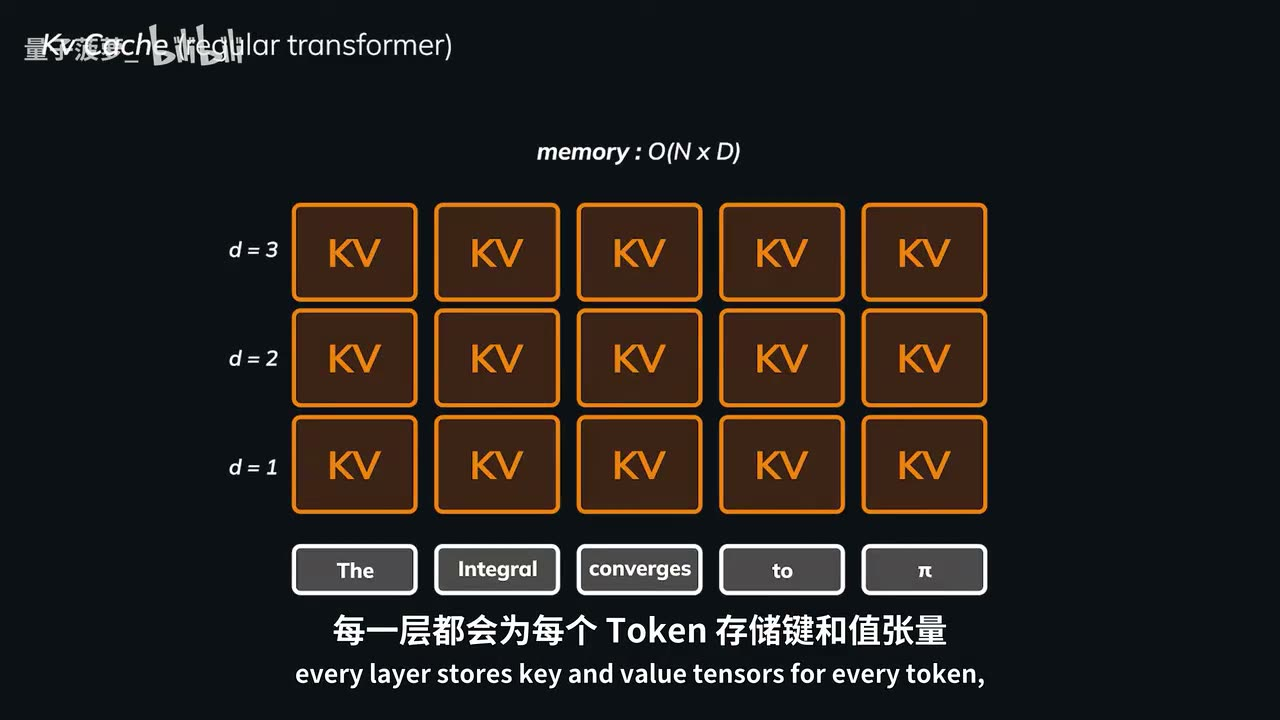
\includegraphics[width=0.82\linewidth,height=0.36\textheight,keepaspectratio]{figures/fig_13_recursive_kv_cache.jpg}
  \caption{朴素递归模型的 KV cache 压力：共享参数减少了权重副本，递归深度仍可能引入多份 KV 状态。\protect\footnotemark}
  \label{fig:recursive-kv-cache}
\end{figure}
\footnotetext{视频画面时间区间：00:12:59--00:13:20。}

\subsection{朴素递归缓存的放大}

先用一句白话说明公式要表达的东西：如果每个 token 在每个递归深度都留下独立 KV，那么缓存大小会同时随上下文 token 数和递归步数增长。递归深度 \(R\) 省下的是同一模块的参数副本，未必省下每一步产生的状态副本。

$$
M_{\mathrm{naive}}\propto nR d_{\mathrm{model}}
$$

\begin{itemize}
  \item \(M_{\mathrm{naive}}\)：朴素递归 KV 缓存的近似内存量。
  \item \(n\)：当前上下文中的 token 数。
  \item \(R\)：最大递归深度，也就是共享模块最多被重复应用的次数。
  \item \(d_{\mathrm{model}}\)：每个 token 表示的模型维度；真实系统还会乘上层数、注意力头数、K/V 两份张量和数值精度字节数。
  \item \(\propto\)：表示只看主导比例关系，省略实现相关常数。
\end{itemize}

这个式子的工程含义很硬：循环架构省参数，缓存系统仍可能要为 \(n\times R\) 个状态服务。在长上下文解码中，GPU 计算单元经常等待显存读写；此时 FLOPs 账面节省无法直接转化成吞吐提升。

\begin{warningbox}{部署评估提醒}
评估循环模型时，单看参数量和理论计算量容易误判。真实服务还要测每 token 延迟、批处理吞吐、显存峰值、KV 读写带宽和缓存命中形态。递归让计算更紧凑，也可能让状态管理更复杂。
\end{warningbox}

\subsection{递归感知缓存：只为活跃 token 付费}

递归感知缓存（recursion-aware cache）的思路是让缓存跟着 MoR 的自适应递归走：已经提前退出的 token 停止产生更深递归的 KV，仍在思考的 token 继续保留当前步所需的 key/value。这样，越往深处走，活跃 token 数 \(n_t\) 越少，缓存和 attention 计算随之收缩。

这条公式表达的是“每一层递归只为仍活跃的 token 保存状态”，所以总内存由各递归步的活跃 token 数累加决定。

$$
M_{\mathrm{aware}}\propto \sum_{t=1}^{R} n_t d_{\mathrm{model}},\qquad n_{t+1}\le n_t
$$

\begin{itemize}
  \item \(M_{\mathrm{aware}}\)：递归感知缓存的近似内存量。
  \item \(t\)：递归步编号。
  \item \(R\)：最大递归深度。
  \item \(n_t\)：第 \(t\) 次递归仍处于活跃状态的 token 数。
  \item \(d_{\mathrm{model}}\)：每个 token 的表示维度。
  \item \(n_{t+1}\le n_t\)：表示 token 可以提前退出，所以后续递归的活跃集合通常不增大。
\end{itemize}

递归感知缓存的优势来自“新鲜”：每一步都使用当前递归步更新后的表示来生成 KV。它更符合模型正在逐步修正隐藏状态的事实，质量通常更稳。代价也清楚：仍活跃的 token 会在多个深度保留新版本 KV，显存占用和缓存写入量高于最激进的共享方案。

\subsection{递归 KV 共享：省内存的代价是表示变旧}

递归 KV 共享（recursive KV sharing）进一步压缩缓存：模型在较早递归步生成 KV，后续递归复用这份缓存，减少跨递归深度复制。直觉上，它像拍下第一轮草稿的索引快照，后面多轮修改时继续查这份快照。这样显存更省，隐藏状态的最新变化也更难完整反映到 attention 读写中。

用最简化形式表示，递归共享把深度维度从缓存主项中拿掉，使缓存近似随 token 数增长。

$$
M_{\mathrm{share}}\propto n d_{\mathrm{model}}
$$

\begin{itemize}
  \item \(M_{\mathrm{share}}\)：递归 KV 共享的近似内存量。
  \item \(n\)：上下文 token 数。
  \item \(d_{\mathrm{model}}\)：每个 token 表示的模型维度。
  \item 省略的常数：层数、头数、K/V 两份张量、数值精度和具体缓存布局。
\end{itemize}

\begin{figure}[htbp]
  \centering
  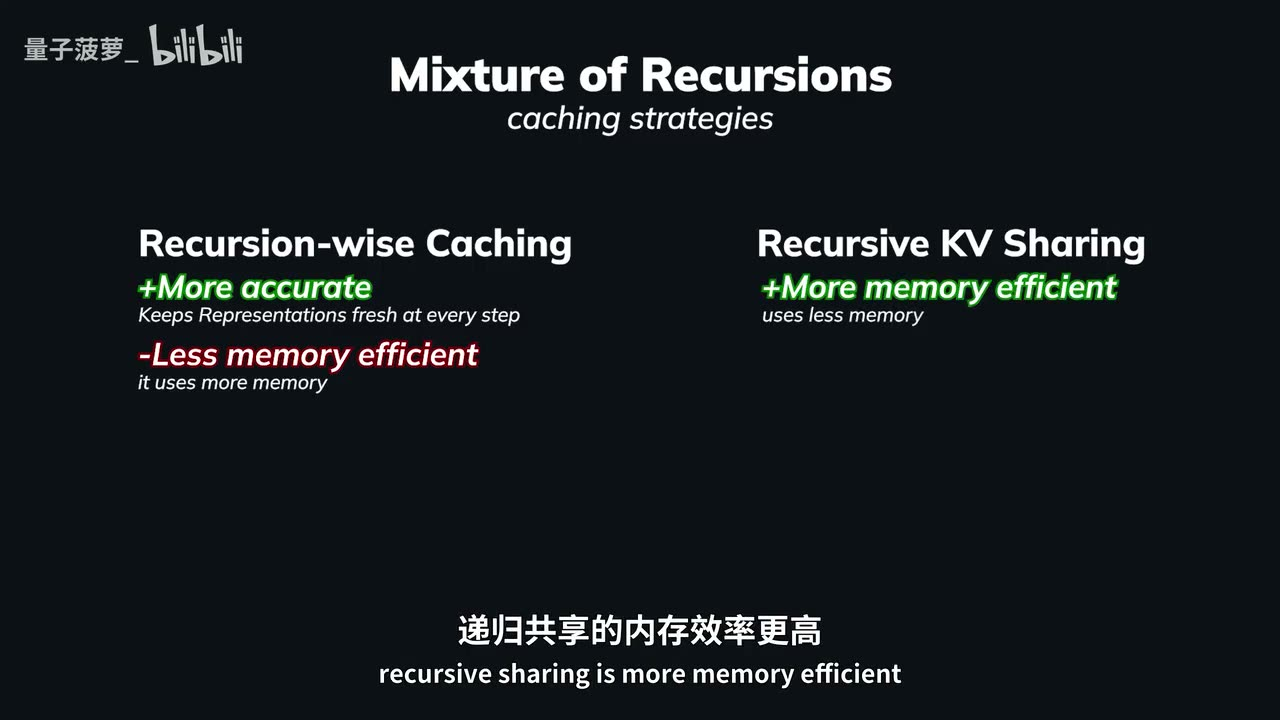
\includegraphics[width=0.82\linewidth,height=0.36\textheight,keepaspectratio]{figures/fig_14_mor_cache_tradeoff.jpg}
  \caption{MoR 缓存策略的权衡：递归感知缓存保持表示新鲜，递归 KV 共享更节省内存。\protect\footnotemark}
  \label{fig:mor-cache-tradeoff}
\end{figure}
\footnotetext{视频画面时间区间：00:14:15--00:14:25。}

因此，缓存策略的核心取舍是内存效率和表示新鲜度。递归感知缓存更适合质量优先或活跃 token 很快减少的场景；递归 KV 共享更适合显存紧张、带宽敏感、可以接受少量质量折损的场景。视频里提到这些权衡在论文实验中可控，并且和自适应路由结合后有机会优于朴素递归模型与标准 Transformer；这个判断仍需要在具体任务、上下文长度和服务批量下重新测量。

\subsection{本章小结}

KV cache 把 Loop Transformer 从“架构参数问题”带回“推理系统问题”。本章应带走三点：

\begin{itemize}
  \item 共享参数降低权重存储，不保证降低每步 attention 状态的内存流量。
  \item 朴素递归缓存的压力近似随 \(nR\) 增长，长上下文会把显存和带宽瓶颈放大。
  \item 递归感知缓存用更多新鲜 KV 换质量，递归 KV 共享用较旧 KV 换内存效率；两者都属于工程权衡，需要用真实延迟、吞吐和质量指标一起评估。
\end{itemize}
